\begin{knitrout}
\definecolor{shadecolor}{rgb}{1, 1, 1}\color{fgcolor}\begin{kframe}
\begin{alltt}
\hlstd{x} \hlkwb{<-} \hlkwd{read.csv}\hlstd{(}\hlstr{"data/stockres.txt"}\hlstd{)}
\hlstd{x} \hlkwb{<-} \hlkwd{unlist}\hlstd{(x)}
\hlcom{# Eliminar nombres de las columnas}
\hlkwd{names}\hlstd{(x)} \hlkwb{<-} \hlkwa{NULL}

\hlstd{u} \hlkwb{<-} \hlkwd{seq}\hlstd{(}\hlopt{-}\hlnum{0.15}\hlstd{,} \hlnum{0.15}\hlstd{,} \hlkwc{by} \hlstd{=} \hlnum{0.01}\hlstd{)}

\hlstd{mu} \hlkwb{<-} \hlkwd{mean}\hlstd{(x)}
\hlstd{sigma} \hlkwb{<-} \hlkwd{sd}\hlstd{(x)}

\hlstd{f_param} \hlkwb{<-} \hlkwd{dnorm}\hlstd{(u,} \hlkwc{mean} \hlstd{= mu,} \hlkwc{sd} \hlstd{= sigma)}

\hlstd{h} \hlkwb{<-} \hlnum{0.02}

\hlstd{n_bins} \hlkwb{<-} \hlkwd{floor}\hlstd{(}\hlkwd{diff}\hlstd{(}\hlkwd{range}\hlstd{(x))} \hlopt{/} \hlstd{h)}

\hlstd{f_hist} \hlkwb{<-} \hlkwd{hist}\hlstd{(x,} \hlkwc{breaks} \hlstd{= n_bins)}
\end{alltt}
\end{kframe}
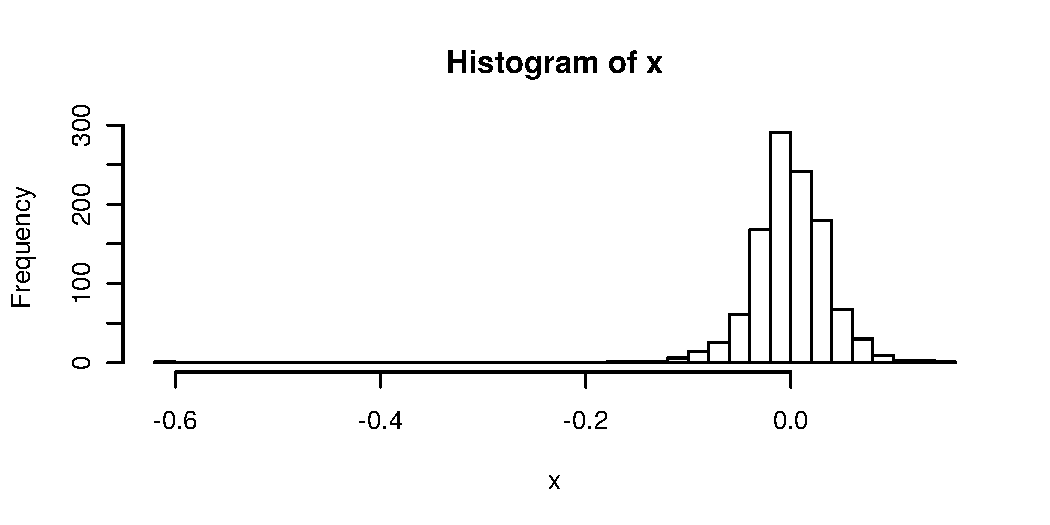
\includegraphics[width=\maxwidth]{figure/unnamed-chunk-21-1} 
\begin{kframe}\begin{alltt}
\hlstd{f_epa} \hlkwb{<-} \hlkwd{as.data.frame}\hlstd{(}\hlkwd{bkde}\hlstd{(x,} \hlkwc{kernel} \hlstd{=} \hlstr{"epa"}\hlstd{,} \hlkwc{bandwidth} \hlstd{= h))}

\hlstd{x_df} \hlkwb{<-} \hlkwd{data.frame}\hlstd{(x)}

\hlkwd{library}\hlstd{(ggplot2)}

\hlkwd{ggplot}\hlstd{(x_df,} \hlkwd{aes}\hlstd{(x))} \hlopt{+}
 \hlkwd{geom_histogram}\hlstd{(}
   \hlkwd{aes}\hlstd{(}\hlkwc{y} \hlstd{= ..density..),}
   \hlkwc{binwidth} \hlstd{=} \hlnum{0.02}\hlstd{,}
   \hlkwc{col} \hlstd{=} \hlstr{"black"}\hlstd{,}
   \hlkwc{fill} \hlstd{=} \hlstr{"white"}
 \hlstd{)} \hlopt{+}
 \hlkwd{stat_function}\hlstd{(}
   \hlkwc{fun} \hlstd{= dnorm,}
   \hlkwc{args} \hlstd{=} \hlkwd{list}\hlstd{(}\hlkwc{mean} \hlstd{= mu,} \hlkwc{sd} \hlstd{= sigma),}
   \hlkwc{color} \hlstd{=} \hlstr{"red"}
 \hlstd{)} \hlopt{+}
 \hlkwd{geom_line}\hlstd{(}\hlkwc{data} \hlstd{= f_epa,} \hlkwd{aes}\hlstd{(x, y),} \hlkwc{color} \hlstd{=} \hlstr{"blue"}\hlstd{)} \hlopt{+}
 \hlkwd{theme_minimal}\hlstd{(}\hlkwc{base_size} \hlstd{=} \hlnum{20}\hlstd{)}
\end{alltt}
\end{kframe}
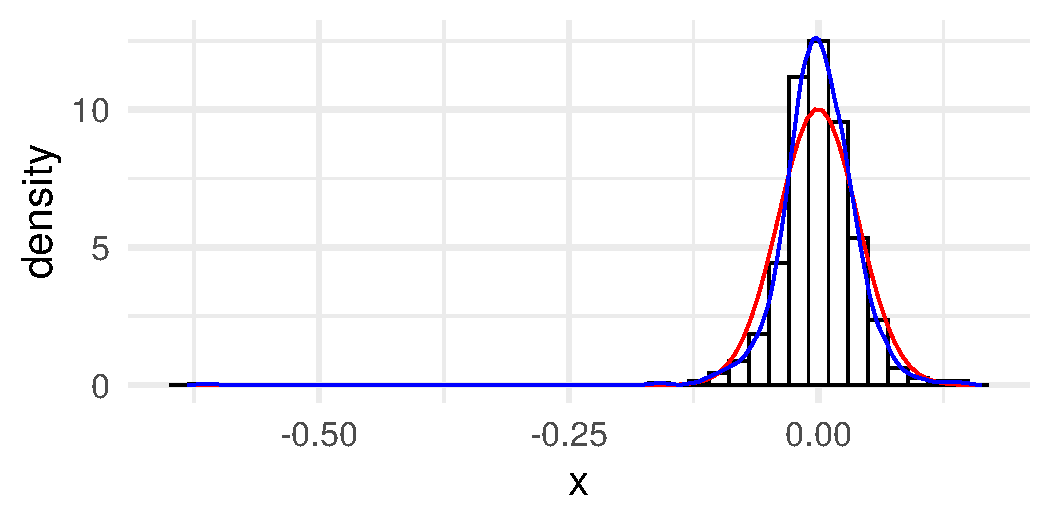
\includegraphics[width=\maxwidth]{figure/unnamed-chunk-21-2} 

\end{knitrout}
